\documentclass{beamer}

\usepackage[utf8]{inputenc}
\usepackage[english]{babel}

\usepackage{graphicx}
\usepackage{amsmath}
\usepackage{amssymb}
\usepackage{amsthm}
\usepackage{array}

\usepackage{alltt}

\addtocounter{footnote}{1}
\setcounter{tocdepth}{5}
\setcounter{secnumdepth}{5}
\renewcommand{\floatpagefraction}{0.75}

%Information to be included in the title page:
\title{Shading with OpenGL 3.3}
\author{Alexander Christensen}
\institute{Department of Computer Science \\ University of Copenhagen}
\date{2018}

%% Reference an equation, a figure, or a section

%% \secref{label} - make a reference to a section
\newcommand{\secref}[1]{Section~\ref{#1}}

%% \eqref{reference} - make a reference to an equation
%%\newcommand{\eqref}[1]{(\ref{#1})}

%% \figref{reference} - make a reference to an figure
\newcommand{\figref}[1]{Figure~\ref{#1}}

\newcommand{\basetop}[1]{\vtop{\vskip-1ex\hbox{#1}}}
\newcommand{\source}[1]{\let\thefootnote\relax\footnotetext{\scriptsize\textcolor{kugray1}{Source: #1}}}

\bibliographystyle{longalpha}
\bibliography{./ref}

%% -*- Mode: latex -*-

%% Macros defined during a long time and used much
% plus - a plus sign
\newcommand{\plus}{+}

% minus - a minus having the same width as a plus
\newlength{\minuswidth}
\settowidth{\minuswidth}{+}
\newlength{\minusheight}
\settoheight{\minusheight}{+}
\newcommand{\minus}{\rule[0.5\minusheight]{\minuswidth}{0.5pt}}

% The basis vector standard
%\renewcommand{\vec}[1]{\boldsymbol{#1}}
\newcommand{\grad}{\operatorname{\nabla}}
\newcommand{\curl}{\operatorname{\text{curl}}}
\newcommand{\divergence}{\operatorname{\text{div}}}
\newcommand{\vecop}{\operatorname{\text{vec}}}
\newcommand{\diag}{\operatorname{\text{diag}}}
\renewcommand{\Re}{\mathbb{R}}
\newcommand{\Co}{\mathbb{C}}
\newcommand{\In}{\mathbb{Z}}
\newcommand{\sign}{\operatorname{sgn}}
%\newcommand{\trace}{\operatorname{Tr}}
\newcommand{\arctantwo}{\ensuremath{\arctan\!2}}
%\newcommand{\mat}[1]{\ensuremath{\boldsymbol{#1} }}
\newcommand{\I}{\mat{1}}
\newcommand{\crossmat}[1]{\ensuremath{\boldsymbol{#1}^{\times} }}
\newcommand{\jacobian}[1]{\ensuremath{\boldsymbol{\mathit{#1}} }}
\newcommand{\set}[1]{\ensuremath{ \boldsymbol{#1} }}
\newcommand{\func}[1]{{\bf{#1}}}
\newcommand{\enorm}[1]{\ensuremath{\left\| #1 \right\|_{_2}}}
%\newcommand{\norm}[1]{\ensuremath{\left\| #1 \right\|}}
\newcommand{\bdet}[1]{\ensuremath{\left| #1 \right|}}
\newcommand{\abs}[1]{\ensuremath{\left| #1 \right|}}
\newcommand{\rtm}{$^{\textrm{®}}$}


\newcommand{\kenny}[1]{ #1 }
\newcommand{\henrik}[1]{ #1 }


%% \maya - the maya signature
\newcommand{\maya}{$ \texttt{Maya}^{\text{\texttrademark}} $}

%% \fat{symbol} - make this symbol fat
\newcommand{\fat}[1]{\mathit{\mathbf{#1}}}
%% \newcommand{\fat}[1]{\hbox{\boldmath $ #1 $}}

%% \vec{symbol} - Vector
%% \renewcommand{\vec}[1]{\mathbf{#1}}
\renewcommand{\vec}[1]{\fat{#1}}

%% \mat{symbol} - Matrix
%%\newcommand{\mat}[1]{\ensuremath{\boldsymbol{#1} }}
\newcommand{\mat}[1]{\fat{#1}}

%% \ezero,...,\ethree - the spin matrices
\newcommand{\ezero}{\begin{bmatrix} 1 & 0 \\  0 &  1 \end{bmatrix}}
\newcommand{\eone}{\begin{bmatrix} i & 0 \\  0 & -i \end{bmatrix}}
\newcommand{\etwo}{\begin{bmatrix} 0 & 1 \\ -1 &  0 \end{bmatrix}}
\newcommand{\ethree}{\begin{bmatrix} 0 & i \\  i &  0 \end{bmatrix}}

%% \quat{symbol} - Quaternion
%% \newcommand{\quat}[1]{\mathbf{#1}}
\newcommand{\quat}[1]{\fat{#1}}

%% \real{quaternion} - the real (scalar) part of a quaternion
\newcommand{\real}{\operatorname{real}}

%% \pure{quaternion} - the pure (vector) part of a quaternion
\newcommand{\pure}{\operatorname{pure}}

%% \sgn{symbol} - the sign of a symbol
\newcommand{\sgn}{\operatorname{sgn}}

%% \norm{symbol} - Norm of a vector/quaternion
\newcommand{\norm}[1]{\parallel {#1} \parallel}

%% \trace{matrix}
\newcommand{\trace}[1]{\mathrm{trace}(#1)}

% This is for code-snippets in the text.
\usepackage{fancyvrb}   %% Try to comment this out if problems with pdflatex
\newcommand{\code}[1]%
%{ \VerbatimInput[frame=none,fontsize=\footnotesize,numbers=none,label=\texttt{#1}]{#1}  }
{ \VerbatimInput[frame=single,fontsize=\footnotesize,numbers=left,label=\texttt{#1}]{#1}  }


%\newcommand{\todo}[1]{ {\Bf Todo:} #1}
\newcommand{\todo}[1]{ }

%\newcommand{\longversion}[1]{ #1 }
\newcommand{\longversion}[1]{ }


\mode<presentation>
{
  \usetheme{Diku}
  \beamertemplatenavigationsymbolsempty
  \setbeamercovered{invisible}
%  \setbeamercovered{transparent=15}
}

%% Kennys pseudocode environment

\newenvironment{pseudocode}{
  \begin{center}
    \begin{minipage}[t]{0.8\columnwidth}
      \footnotesize
      \rule{\columnwidth}{1pt}
    }{
      \rule{\columnwidth}{1pt}
    \end{minipage}
  \end{center}
}

{
\AtBeginSection[wef]
{
\begin{frame}
\frametitle{Table of Contents}
\tableofcontents[currentsection]{1}
\end{frame}
}
}





\begin{document}

% Set background to front page
\usebackgroundtemplate{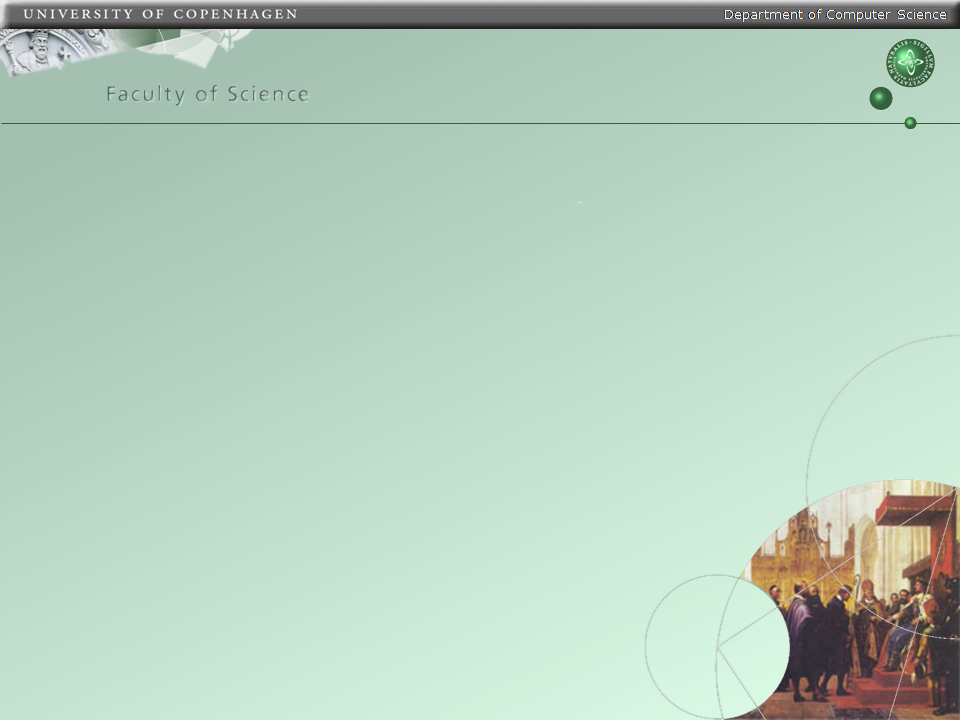
\includegraphics[width=\paperwidth,height=\paperheight]{front}}
{
\begin{frame}[plain]
  \titlepage
\end{frame}
}

% Set background to rest of pages
\usebackgroundtemplate{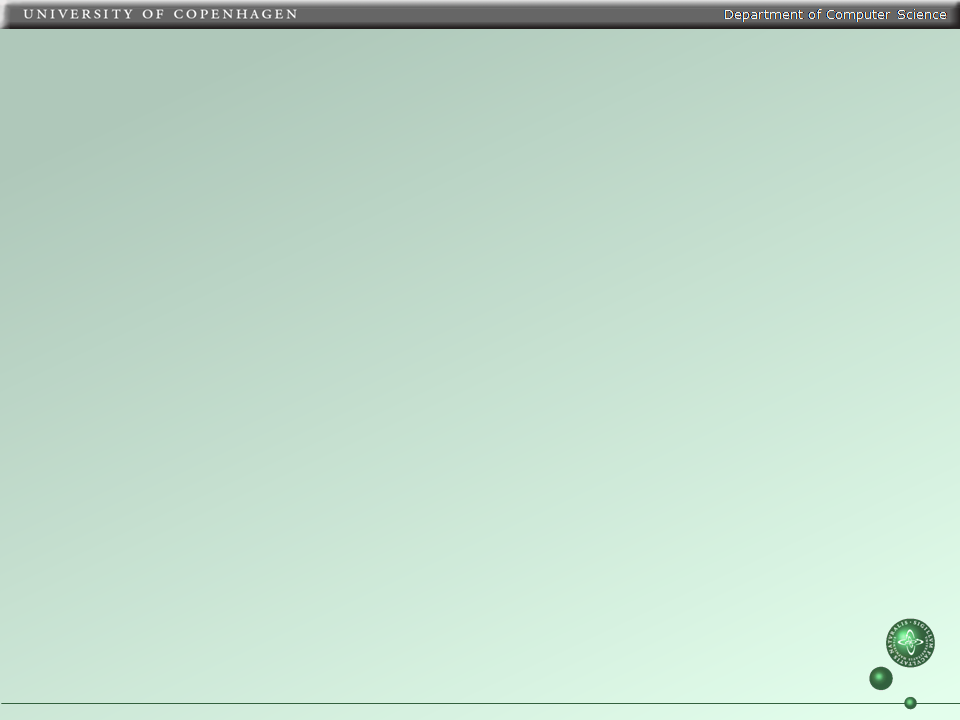
\includegraphics[width=\paperwidth,height=\paperheight]{background}}

%
%
%
\begin{frame}
\frametitle{Overview}
\tableofcontents
%% This is a text in first frame. This is a text in first frame. This is a text in first frame.
\end{frame}


%
%
%
\section{Shading pipeline}

\begin{frame}
\frametitle{Shading pipeline}

TODO: Include pipeline picture!

Where are the scan conversion algorithms run?

What is rasterization?

What is a shader?
\end{frame}


%
%
%
\section{glsl - OpenGL Shading Language}

\begin{frame}
\frametitle{glsl - OpenGL Shading Language}

History with OpenGL (fixed-function pipeline vs. programmable shaders)

glsl is a DSL for writing programmable shaders

glsl has a C-like language syntax

Shaders are purely run on the GPU!
\end{frame}


%
%
%
\begin{frame}
\frametitle{glsl - OpenGL Shading Language}
Supported expressions:

\begin{itemize}
\item primitive data types: \texttt{float, int, uint, $\ldots$}
\item vector/matrix data types: \texttt{mat2, mat3, mat4, vec2, vec3, vec4, $\ldots$}
\item special types: \texttt{struct, enum}
\item functions
\end{itemize}

\end{frame}


%
%
%
\begin{frame}
\frametitle{glsl - OpenGL Shading Language}

\subsection{Runtime requirements}
Important guarantee: determinable running time!

\begin{itemize}
\item No while loops
\item No recursion
\end{itemize}

\subsection{Ensure parallelism}
\underline{Remarks:}\\\vspace{1mm}
Shader execution calls are independent and run in parallel

Not possible to read/modify return values of other shader calls in shader code

Execution units on GPU's typically cannot do branch-prediction very well!
\end{frame}


%
%
%
\section{Shader programs}

\subsection{Vertex shader}
\begin{frame}
\frametitle{Shader programs - Vertex shader}

Per-vertex processing

Built-in variables: \texttt{gl\_Position}

Can modify position.

Outputs a vertex position which must be in normalized coordinates (NDC)
\end{frame}


%
%
%
\subsection{Fragment shader}
\begin{frame}
\frametitle{Shader programs - Fragment shader}
Per-fragment processing.

Each fragment is typically the size of a pixel

Built-in variables: \texttt{gl\_FragCoord, gl\_FrontFacing, gl\_PointCoord}

Outputs a color value (r, g, b, a), in normalized coordinates ($[0, 1]$).

\end{frame}


%
%
%
\begin{frame}
\frametitle{Shader variables - Attributes}

Attributes are used in vertex shaders:

\begin{alltt}\footnotesize
layout (location = 0) in vec3 vertexPosition;\\
layout (location = 1) in vec2 texCoord;
\end{alltt}

Data, such as vertex positions, are buffered to the GPU.

Attributes are pointers to this data.

\begin{alltt}
GLfloat data[] = \{\\
    // vertexPosition \ensuremath{\quad} texCoord\\
    0.0f, 0.5f, -0.3f,\ensuremath{\quad}    0.0f, 0.0f,\\
    //  ...\\
\}
\end{alltt}

\end{frame}


%% \begin{frame}
%% \frametitle{Shader variables - Uniforms}
%% \end{frame}

%% \begin{frame}
%% \frametitle{Shader variables - input/ouput}
%% \end{frame}

%% \begin{frame}
%% \frametitle{Shader variables - interpolation qualifiers}
%% \end{frame}

%
%
%
\begin{frame}
\frametitle{How many times is it run?}

Imagine a triangle, in NDC, with coordinates $(-1,-1,0), (-1,1,0), (1,1,0)$.

Assume application window of size $800 \times 600$

$\rightarrow \quad$ 3 vertex shader calls

$\rightarrow \quad \approx (800\cdot 600) / 2\ =\ $ 240000 fragment shader calls!
\end{frame}


%
%
%
\begin{frame}
\frametitle{Creating a shader program}
\end{frame}

\begin{frame}
\frametitle{Debugging}
Black screen

Check variables before they are sent to the GPU
\end{frame}


%
%
%
\section{Examples}

\begin{frame}
\frametitle{Example 1 - static rendering}
\end{frame}

\begin{frame}
\frametitle{Example 2 - animation}
\end{frame}

\begin{frame}
\frametitle{Summary}
\end{frame}

\begin{frame}
\frametitle{References}
\end{frame}

%\footnotesize
\bibliography{refs}

\end{document}
